%% 
%% Copyright 2007-2025 Elsevier Ltd
%% 
%% This file is part of the 'Elsarticle Bundle'.
%% ---------------------------------------------
%% 
%% It may be distributed under the conditions of the LaTeX Project Public
%% License, either version 1.3 of this license or (at your option) any
%% later version.  The latest version of this license is in
%%    http://www.latex-project.org/lppl.txt
%% and version 1.3 or later is part of all distributions of LaTeX
%% version 1999/12/01 or later.
%% 
%% The list of all files belonging to the 'Elsarticle Bundle' is
%% given in the file `manifest.txt'.
%% 
%% Template article for Elsevier's document class `elsarticle'
%% with numbered style bibliographic references
%% SP 2008/03/01
%% $Id: elsarticle-template-num.tex 272 2025-01-09 17:36:26Z rishi $
%%
\documentclass[preprint,12pt]{elsarticle}

%% Use the option review to obtain double line spacing
%% \documentclass[authoryear,preprint,review,12pt]{elsarticle}

%% Use the options 1p,twocolumn; 3p; 3p,twocolumn; 5p; or 5p,twocolumn
%% for a journal layout:
%% \documentclass[final,1p,times]{elsarticle}
%% \documentclass[final,1p,times,twocolumn]{elsarticle}
%% \documentclass[final,3p,times]{elsarticle}
%% \documentclass[final,3p,times,twocolumn]{elsarticle}
%% \documentclass[final,5p,times]{elsarticle}
%% \documentclass[final,5p,times,twocolumn]{elsarticle}

%% For including figures, graphicx.sty has been loaded in
%% elsarticle.cls. If you prefer to use the old commands
%% please give \usepackage{epsfig}

%% The amssymb package provides various useful mathematical symbols
%% The amsmath package provides various useful equation environments.

%% The amsthm package provides extended theorem environments
%% \usepackage{amsthm}

%% The lineno packages adds line numbers. Start line numbering with
%% \begin{linenumbers}, end it with \end{linenumbers}. Or switch it on
%% for the whole article with \linenumbers.
%% \usepackage{lineno}

\usepackage{natbib}
\usepackage{amsmath,amssymb,amsfonts}
\usepackage{graphicx}
\usepackage{amsthm}
\usepackage{textcomp}
\usepackage{booktabs}
\usepackage{multirow}
\usepackage{algorithm}
\usepackage{algpseudocode}
\usepackage{pifont}
\usepackage{ragged2e}
\usepackage{float}
\usepackage{array}
\usepackage{adjustbox}

\journal{Blockchain: Research and Applications}

\begin{document}

\begin{frontmatter}

%% Title, authors and addresses

%% use the tnoteref command within \title for footnotes;
%% use the tnotetext command for theassociated footnote;
%% use the fnref command within \author or \affiliation for footnotes;
%% use the fntext command for theassociated footnote;
%% use the corref command within \author for corresponding author footnotes;
%% use the cortext command for theassociated footnote;
%% use the ead command for the email address,
%% and the form \ead[url] for the home page:
%% \title{Title\tnoteref{label1}}
%% \tnotetext[label1]{}
%% \author{Name\corref{cor1}\fnref{label2}}
%% \ead{email address}
%% \ead[url]{home page}
%% \fntext[label2]{}
%% \cortext[cor1]{}
%% \affiliation{organization={},
%%             addressline={},
%%             city={},
%%             postcode={},
%%             state={},
%%             country={}}
%% \fntext[label3]{}

\title{Can Taproot-Based Commitments Enable Scalable and Revocable Document Verification in Distributed Communication Networks?}

%% use optional labels to link authors explicitly to addresses:
%% \author[label1,label2]{}
%% \affiliation[label1]{organization={},
%%             addressline={},
%%             city={},
%%             postcode={},
%%             state={},
%%             country={}}
%%
%% \affiliation[label2]{organization={},
%%             addressline={},
%%             city={},
%%             postcode={},
%%             state={},
%%             country={}}


\author[inst1]{Juan Crespo}
\author[inst1]{Sultan Almuhammadi}
\author[inst2]{Moatsum Alawida}
\author[inst1]{Farag Azzedin}

\affiliation[inst1]{organization={Information and Computer Science Department, King Fahd University of Petroleum and Minerals},
city={Dhahran},
country={Saudi Arabia}}

\affiliation[inst2]{organization={Department of Computer Science, Abu Dhabi University},
city={Abu Dhabi},
postcode={59911},
country={United Arab Emirates}}

%% Abstract

\begin{abstract}
Secure verification of digital documents across distributed communication networks requires mechanisms that ensure integrity, authenticity, and efficient revocation while minimizing reliance on centralized verification services. Traditional document verification infrastructures depend on trusted intermediaries and continuous online availability, which introduces scalability constraints and trust limitations in large-scale environments. 
This paper presents a communication-security architecture for distributed document verification based on a Taproot-enabled commitment mechanism anchored in a single Pay-to-Taproot (P2TR) transaction. The proposed framework aggregates document hashes using a Merkle tree structure and embeds the resulting commitment within Taproot, enabling efficient and scalable verification across distributed systems. 
Issuer authenticity is ensured through Schnorr signatures that are cryptographically bound to the commitment, while revocation management is implemented through a transaction chaining mechanism that separates immutable issuance commitments from dynamic revocation states. This design enables lightweight verification, where verifiers exchange compact proofs instead of entire document datasets. 
We provide a formal security analysis under standard cryptographic assumptions and evaluate both communication and verification overhead as functions of the batch size. The results show that Merkle proof size and verification complexity grow logarithmically, $\mathcal{O}(\log N)$, with the number of documents $N$, while the anchoring cost remains constant. 
These findings demonstrate that the proposed architecture offers a scalable and privacy-preserving solution for secure document verification in distributed communication systems, without requiring protocol modifications or reliance on trusted third-party infrastructure.
\end{abstract}

% %%Graphical abstract
% \begin{graphicalabstract}
% %\includegraphics{grabs}
% \end{graphicalabstract}

% %%Research highlights
% \begin{highlights}
% \item Research highlight 1
% \item Research highlight 2
% \end{highlights}

%% Keywords
\begin{keyword}
%% keywords here, in the form: keyword \sep keyword

Bitcoin\sep Taproot\sep  Merkle Commitments\sep Schnorr Signatures\sep Decentralized Document Verification\sep On-chain Revocation\sep Cryptographic Protocols.

%% PACS codes here, in the form: \PACS code \sep code

%% MSC codes here, in the form: \MSC code \sep code
%% or \MSC[2008] code \sep code (2000 is the default)

\end{keyword}
\end{frontmatter}

%% Add \usepackage{lineno} before \begin{document} and uncomment 
%% following line to enable line numbers
%% \linenumbers

%% main text
%%

\section{Introduction}
\label{sec.intro}

Document fraud, particularly involving academic credentials, represents a significant global challenge~\cite{Xie2020EthereumCertificate}. 
Verification of document authenticity, integrity, and validity is traditionally handled by the issuing organizations themselves, creating a structural dependency on centralized verification infrastructures~\cite{shende2024enhancing}. 
Historically, this process has relied on physical mechanisms such as stamps and, more recently, on centralized digital systems maintained by the issuer. 
Even in digital form, centralized verification systems incur significant operational costs in order to maintain availability and to mitigate denial-of-service attacks.

Bitcoin is a decentralized consensus network that maintains a globally replicated ledger through a Proof-of-Work mechanism~\cite{nakamoto2008bitcoin}. 
Its large and sustained computational security budget provides strong resistance against history revision and transaction censorship. 
Because validation is permissionless and globally distributed, Bitcoin offers high availability and long-term immutability guarantees without reliance on centralized infrastructure~\cite{Lemieux2016Trusting}. 
These properties make it a robust substrate for anchoring cryptographic commitments that require durability and public verifiability beyond purely monetary use.

Bitcoin protocol stores only transaction-related data by design, including: amounts, timestamps, and input and output scripts. 
Nevertheless, several approaches have been proposed to anchor external cryptographic commitments in the Bitcoin blockchain in order to support applications such as digital document verification. 
One widely used technique relies on the \texttt{OP\_RETURN} opcode, which allows a limited amount of arbitrary data to be embedded directly in a transaction output. 
Another approach is OpenTimestamps, an open timestamping protocol in which document hashes are aggregated into Merkle trees and periodically anchored in the Bitcoin blockchain by calendar servers operated by third parties. 
In this model, the Merkle tree construction and anchoring transaction are performed externally, and the associated transaction fee is paid by the calendar operator, leaving users without direct control over how batches are formed or when anchoring occurs. 
Blockcerts represents a higher-level framework for issuing and verifying digital credentials, where document hashes are anchored on-chain while certificate metadata is managed off-chain. While this framework enables verifiable credentials, its primary objective is credential representation and management rather than the design of cryptographic commitment structures for decentralized verification.

Despite their usefulness, these approaches remain limited in at least one of three important dimensions: scalable batch aggregation, privacy-preserving per-document verification, or explicit and auditable revocation support. 
In particular, OP\_RETURN-based techniques expose commitment data publicly and do not provide native mechanisms for issuer authentication or document life-cycle management. 
OpenTimestamps enables scalable integrity anchoring but does not address issuer authentication or revocation, while Blockcerts focuses primarily on credential representation rather than on commitment structures designed for decentralized verification.

Recent upgrades to the Bitcoin protocol introduce new capabilities that may help address these limitations. 
In particular, Taproot is a protocol upgrade that combines Schnorr signatures and Merkleized Abstract Syntax Trees (MAST) to enable more efficient and privacy-preserving representation of complex spending conditions on the Bitcoin blockchain.
Taproot introduces a new output type known as Pay-to-Taproot (P2TR), in which coins are locked to a Taproot output key that commits to both a public key and optional script paths encoded through MAST.

The central question addressed in this work is whether Taproot is sufficient to implement a decentralized document verification protocol satisfying scalability, privacy, revocation support, and formally stated security guarantees on Bitcoin.

More precisely, we investigate whether a Taproot-native construction can simultaneously achieve the following:

\begin{enumerate}
    \item Scalable batch aggregation of document commitments,
    \item Privacy-preserving per-document verification,
    \item Explicit and auditable revocation support,
    \item Cryptographic security grounded in formally stated assumptions.
\end{enumerate}

The challenge is to design a construction that satisfies these properties while preserving indistinguishability from standard P2TR outputs and remaining fully compatible with the Bitcoin protocol.

To this end, we introduce a Taproot-native commitment construction that enables batch document verification using a single P2TR transaction. 
The proposed design leverages non-executed Taproot script paths to encode cryptographic commitments, combined with MAST and Schnorr signatures standardized in BIPs~\cite{bip340,bip341}.
Verification is performed entirely off-chain through reconstruction of the Taproot output key and validation of Merkle authentication paths and Schnorr signatures using a proof-of-validation object distributed with each document.

To the best of our knowledge, this work provides one of the first systematic designs of a Taproot-native protocol for decentralized document verification on Bitcoin.

The main contributions of this work are as follows:

\begin{enumerate}
    \item We formalize a Taproot-based commitment structure that embeds document hashes and issuer public keys within non-executed script paths while preserving indistinguishability from standard P2TR outputs.
    
    \item We design a batch document verification protocol that enables per-document integrity and issuer authenticity verification using Merkle authentication paths and Schnorr signatures.
    
    \item We propose a revocation mechanism based on transaction chaining that updates the 
    revocation state without modifying or invalidating the original issuance commitment.
    
    \item We provide an analytical characterization of on-chain transaction cost and off-chain verification complexity as functions of batch size, showing logarithmic $\mathcal{O}(\log N)$ verification complexity and constant anchoring cost.
    
    \item We define a formal security model and provide reduction-based arguments establishing integrity under the collision resistance of the hash function and authenticity under the existential unforgeability under chosen-message attack (EUF-CMA) of Schnorr signatures, assuming the immutability of the Bitcoin blockchain.
\end{enumerate}


\section{Related Work}
\label{sec.relatedwork}

This section reviews prior work on information anchoring techniques in the Bitcoin blockchain and on the use of smart contracts in Ethereum, with a focus on their application to document verification systems and their limitations in terms of scalability, privacy, and revocation support.

\subsection{Information Anchoring Techniques in Bitcoin}
\label{sec.methodsbitcoin}

The Bitcoin protocol adopts a deliberately restrictive execution model based on the Unspent Transaction Output (UTXO) abstraction and a non-Turing-complete scripting language.
Scripts have no access to persistent state, arbitrary function calls, or iterative control structures, which constrains the design space for data anchoring and commitment mechanisms.
These architectural restrictions directly impact how document verification systems can be implemented at the base layer.

Early data anchoring approaches encoded arbitrary bytes into payment addresses, effectively embedding metadata within transaction outputs~\cite{Gao2017Decentralized}.
These methods incur linear on-chain growth with batch size, permanently lock bitcoin in unspendable outputs, and introduce unnecessary UTXO set expansion.
As a result, fake address-based schemes are economically inefficient and do not scale for structured document verification systems.

With the introduction of additional payment script types, alternative data anchoring techniques have been proposed.
Comprehensive analyses classify these approaches into two main categories: script-based methods, which increase construction and verification complexity, and fake address-based methods, which incur higher cost and lack privacy~\cite{Bartoletti2019BitcoinMetadata}.
Among these, OP\_RETURN-based techniques explicitly mark outputs as unspendable and avoid UTXO set growth, thereby reducing negative impact on the network~\cite{Strehle2020DominatingOPReturns}.
While OP\_RETURN has historically been constrained by policy limits, it remains the most widely adopted mechanism for anchoring non-monetary data in Bitcoin.

The introduction of Segregated Witness (SegWit) reorganized transaction structure by isolating witness data and applying discounted weight to signature material, reducing effective transaction cost~\cite{Kedziora2022AnalysisSegWit}.
This enabled lower-cost commitment schemes that leverage witness fields for data anchoring.
However, SegWit-based techniques remain limited to integrity anchoring and do not natively support issuer authentication, explicit revocation, or structured batch verification within a unified design.

Several standardized solutions are widely deployed on Bitcoin today.
Blockcerts~\cite{Blockcerts} and OpenTimestamps~\cite{OpenTimestamps} are representative Bitcoin-based systems for credential anchoring and timestamping, respectively. 
However, both remain primarily integrity-oriented and do not provide a Taproot-native mechanism that cryptographically couples issuer authenticity and revocation to the anchoring output itself.

Table~\ref{tab:comp_functional} summarizes the functional properties supported by representative Bitcoin-based document anchoring techniques. 
The comparison focuses on key capabilities relevant for document verification systems, including batch commitments, issuer authentication, revocation support, privacy preservation, and independent verification. 
Early techniques such as Fake Address and OP\_RETURN primarily provide document integrity by anchoring hashes directly on-chain, but they lack mechanisms for issuer authentication and lifecycle management. 
Script and witness-based constructions improve flexibility but remain integrity-oriented. 
OpenTimestamps introduces scalable batch commitments through Merkle aggregation; however, it does not natively provide issuer authentication or explicit revocation mechanisms. 
In contrast, the proposed Taproot-based construction integrates batch commitments, issuer authenticity, and revocation support within a unified protocol design.

\begin{table}[t]
\caption{Functional comparison of existing Bitcoin anchoring approaches and the proposed Taproot-based protocol.}
\label{tab:comp_functional}
\centering
\small
\renewcommand{\arraystretch}{1.3}

\begin{adjustbox}{max width=\linewidth}
\begin{tabular}{
>{\centering\arraybackslash}m{3cm}
c c c c
>{\centering\arraybackslash}m{2.8cm}
>{\centering\arraybackslash}m{2.6cm}
}
\toprule
\textbf{Property} &
\textbf{Fake Address} &
\textbf{OP\_RETURN} &
\textbf{Script} &
\textbf{Witness} &
\shortstack{\textbf{OpenTimestamps}\\(OTS)} &
\shortstack{\textbf{Proposed}\\(Taproot)} \\
\midrule

Integrity Verification &
\ding{51} & \ding{51} & \ding{51} & \ding{51} & \ding{51} & \ding{51} \\

Issuer Authentication &
\ding{55} & \ding{55} & \ding{55} & \ding{55} & \ding{55} & \ding{51} \\

Document Revocation &
\ding{55} & \ding{55} & \ding{55} & \ding{55} & \ding{55} & \ding{51} \\

Batch Support &
\ding{55} & \ding{55} & \ding{55} & \ding{55} & \ding{55} & \ding{51} \\

Privacy &
\ding{55} & LOW & HIGH & HIGH & MEDIUM & HIGH \\

\bottomrule
\end{tabular}
\end{adjustbox}

\end{table}

Table~\ref{tab:comparative_cost} compares the computational and on-chain efficiency of different Bitcoin anchoring approaches. 
The evaluation considers transaction footprint, batching efficiency, and verification overhead. 
Legacy techniques such as Fake Address and OP\_RETURN incur linear on-chain growth because each document requires an individual commitment. 
Script and witness-based approaches improve fee efficiency but still scale linearly with the number of documents. 
OpenTimestamps reduces the on-chain footprint by aggregating document hashes into a Merkle tree, enabling constant anchoring cost and logarithmic verification proofs. 
The proposed Taproot-based construction preserves these scalability properties while integrating issuer authentication and revocation support within the same commitment structure.

\begin{table}[t]
\caption{Network impact and transaction cost characteristics of Bitcoin-based document anchoring approaches.}
\label{tab:comparative_cost}
\centering
\small
\renewcommand{\arraystretch}{1.6}

\begin{adjustbox}{max width=\linewidth}
\begin{tabular}{
>{\centering\arraybackslash}m{3.2cm}
c c c c
>{\centering\arraybackslash}m{2.8cm}
>{\centering\arraybackslash}m{2.8cm}
}
\toprule
\textbf{Property} &
\textbf{Fake Address} &
\textbf{OP\_RETURN} &
\textbf{Script} &
\textbf{Witness} &
\shortstack{\textbf{OpenTimestamps}\\(OTS)} &
\shortstack{\textbf{Proposed}\\(Taproot)} \\
\midrule

On-chain footprint &
HIGH & LOW & HIGH & MEDIUM & LOW & LOW \\

UTXO impact &
HIGH & NONE & LOW & LOW & LOW & LOW \\

TX Cost Model (BTC) &
\shortstack{Burn\\+ fee} &
\shortstack{Standard\\fee} &
\shortstack{Standard\\fee} &
\shortstack{Discounted\\SegWit} &
\shortstack{Shared\\anchoring} &
\shortstack{Discounted\\SegWit} \\

Verification efficiency &
LOW & LOW & LOW & LOW & LOW & HIGH \\

Size (bytes) &
$20\times N$ &
$\sim 80$ &
$\sim 1000$ &
$\sim 4000$ &
$\sim 40$--$80$ &
$\sim 32$ \\

\bottomrule
\end{tabular}
\end{adjustbox}

\end{table}

Due to Bitcoin’s intentionally restricted execution model, many document verification systems have migrated toward more expressive blockchain platforms. Ethereum introduces an account-based state model and a Turing-complete virtual machine that enables persistent storage and arbitrary contract logic~\cite{buterin2014ethereum}. This architectural difference allows on-chain verification and revocation logic to be implemented directly within smart contracts, but introduces higher execution complexity, gas-based cost variability, and a broader attack surface. Table~\ref{tab:btc_eth_comparison} summarizes the architectural and security differences between Bitcoin and Ethereum in the context of document verification systems.

\begin{table}[t]
\caption{Condensed architectural and security comparison between Bitcoin and Ethereum for document verification systems.}
\label{tab:btc_eth_comparison}
\centering
\small
\renewcommand{\arraystretch}{1.2}
\setlength{\tabcolsep}{4pt}

\begin{adjustbox}{max width=\linewidth}
\begin{tabular}{
>{\raggedright\arraybackslash\bfseries}m{3.0cm}
>{\raggedright\arraybackslash}m{6.2cm}
>{\raggedright\arraybackslash}m{6.2cm}
}
\toprule
Dimension & Bitcoin (PoW, UTXO) & Ethereum (PoS, Account/VM) \\
\midrule

Security basis &
Energy-based security (hashrate $H$) &
Stake-based security (total stake $S$) \\

Adversarial threshold &
$\alpha = H_A/H_{total}$ &
$\alpha = S_A/S_{total}$ \\

State model &
UTXO; stateless validation &
Global account state; persistent storage \\

Execution model &
Limited, non-Turing Script &
Turing-complete EVM \\

Verification approach &
On-chain commitment, off-chain proof verification &
On-chain contract-based verification \\

Cost model &
Fee per transaction size (vbytes) &
Gas-based fee (computation + storage) \\

Revocation mechanism &
New commitment transaction required &
Contract state update \\

Finality model &
Probabilistic finality &
Economic finality \\

Attack surface &
Minimal scripting layer &
VM and smart-contract dependent \\

Governance style &
Conservative soft-forks &
Frequent hard-fork upgrades \\

\bottomrule
\end{tabular}
\end{adjustbox}

\end{table}

Ethereum enables native on-chain verification through Turing-complete smart contracts and persistent global state, but this flexibility introduces gas-based execution costs, increased systemic complexity, and a broader attack surface. In contrast, Bitcoin relies on a UTXO model with restricted, non-Turing-complete Script, where verification logic is performed off-chain using cryptographic proofs anchored by on-chain commitments. 
Although this model limits computational expressiveness, it reduces execution complexity and minimizes the base-layer attack surface. 
For this reason, this work adopts Bitcoin as the underlying platform, favoring a minimal execution model, predictable fee structure, and strong energy-based security guarantees over contract-dependent on-chain verification.

Numerous studies leverage Ethereum smart contracts to implement certification and attestation systems that require expressive verification logic~\cite{Wang2019BlockchainCT,Li2020DecentralizedPKI,Pennino2021EfficientCertification,Palmisano2022NotarizationAntiPlagiarism,Mishra2025BlockchainDecentralized,Harer2022DecentralizedAttestation}.
While these approaches demonstrate the flexibility of Ethereum’s execution model, they incur increased on-chain execution overhead, higher gas fees, and greater implementation complexity.

Institutional adoption of blockchain-based document verification has also been studied extensively. Castro et al.~\cite{Castro2021BlockchainHigherEducation} analyze blockchain adoption for higher education diplomas.
Rustemi et al.~\cite{Rustemi2023SLRBlockchainCertificates} show that most academic certificate verification platforms are implemented on Ethereum and identify document revocation as a major unresolved challenge.
Recent research further highlights unresolved challenges related to privacy and revocation in decentralized credential systems~\cite{Ramica2024SelectiveDisclosure,Zhang2025PrivacyProtectionIssuanceRevocationVerifiableCredentials}.

\subsection{Limitations of Existing Approaches and Formal Gap}
\label{sec:formal_gap}

Existing Bitcoin-based anchoring mechanisms mainly provide \emph{data integrity} guarantees. However, most of these approaches do not simultaneously support issuer authentication, scalable batch commitments, and explicit revocation within a unified cryptographic framework. Early techniques based on fake addresses and \texttt{OP\_RETURN} embed data directly into Bitcoin transactions. While these approaches are simple to implement, they suffer from practical limitations. In particular, fake-address techniques destroy spendable value, while \texttt{OP\_RETURN}-based methods expose metadata explicitly on-chain, which may reduce privacy and increase blockchain footprint.

OpenTimestamps improves scalability by aggregating document hashes using Merkle trees before anchoring them to the blockchain. Although this approach significantly reduces the number of required transactions, it does not cryptographically bind the commitment to a specific issuer. Moreover, OpenTimestamps does not provide a native mechanism for document revocation. 
Another limitation is that the Merkle aggregation process is typically managed by an external service, which reduces issuer-level control over the commitment structure.

More recent approaches use script- or witness-based constructions, especially after the activation of SegWit. These techniques improve fee efficiency and reduce UTXO growth by placing commitment data in the witness field. Despite these improvements, these solutions remain primarily integrity-oriented and do not provide mechanisms for issuer authentication or lifecycle management of anchored documents.

Ethereum-based certification systems attempt to overcome these limitations by using smart contracts to implement verification and revocation logic directly on-chain. This enables dynamic state updates and explicit revocation tracking.  However, this flexibility comes with several trade-offs, including higher execution complexity, gas-based cost variability, and a broader attack surface due to the use of Turing-complete contract execution. Furthermore, these systems rely on different security assumptions, including contract correctness and economic finality mechanisms.

From a formal perspective, current approaches do not simultaneously achieve the following properties within a purely Bitcoin-native construction:

\begin{itemize}
    \item $\mathcal{O}(1)$ on-chain batch commitment cost,
    \item $\mathcal{O}(\log N)$ per-document verification proof,
    \item cryptographic binding of issuer identity to the on-chain commitment,
    \item explicit and publicly auditable revocation state,
    \item complete off-chain verification without requiring expressive on-chain execution.
\end{itemize}

We consider an adversary capable of: 
(i) forging a document that was not included in the original commitment, 
(ii) presenting a revoked document as valid, or 
(iii) modifying validation proofs. 
The adversary is assumed not to control a majority of the total network hash rate at the time the commitment transaction is confirmed.



In contrast to smart-contract-based approaches, the construction proposed in this work relies exclusively on standardized Bitcoin primitives and off-chain verification. This design avoids on-chain execution overhead while preserving cryptographic verifiability and publicly auditable revocation state transitions. To the best of our knowledge, no prior work systematically leverages Taproot script-path commitments as non-executed commitment carriers within a complete decentralized document verification protocol that explicitly separates issuance and revocation state. The proposed Taproot-based protocol mitigates these limitations by anchoring an issuer-defined Merkle structure within a single P2TR output, achieving $\mathcal{O}(1)$ on-chain batch issuance while maintaining $\mathcal{O}(\log N)$ verification complexity off-chain. Unlike OP\_RETURN or OTS-based methods, it supports native issuer authentication through Schnorr signatures bound to the committed structure and enables explicit revocation via controlled state updates. This design preserves Bitcoin’s minimal trust model while extending its functional capability, achieving scalability, privacy, and semantic completeness without introducing the systemic complexity of general-purpose smart contracts.


%Under these assumptions, the security of the system reduces to the collision resistance of SHA-256 and the EUF-CMA security of Schnorr signatures under BIP340, together with the honest-majority assumption of Nakamoto consensus. To the best of our knowledge, existing works do not formally characterize this design space under explicit security and complexity constraints.




\section{Background}
\label{sec.background}

%\subsection{Bitcoin Script and Transaction Model}

Bitcoin transactions are validated using a script-based execution model that specifies the conditions under which transaction outputs may be spent. 
The Bitcoin protocol follows the UTXO model, where each transaction consumes previously created outputs and generates new ones. Spending conditions are encoded using Bitcoin Script, a stack-based and intentionally non-Turing-complete language designed to guarantee predictable execution complexity and minimize the network's attack surface. 

Bitcoin Script does not support persistent state, loops, or arbitrary function calls. These restrictions enforce deterministic validation and enable decentralized verification even by resource-constrained nodes. Consequently, protocol constructions built on Bitcoin must rely on cryptographic commitments and off-chain verification logic rather than on expressive on-chain stateful computation.

\subsection{Schnorr Signatures in Bitcoin}

With the activation of BIP340, Bitcoin adopted Schnorr digital signatures as the signature scheme for Taproot outputs.
Let $G$ denote the generator of the secp256k1 elliptic curve group of prime order $n$, and let $x \in \mathbb{Z}_n$ denote a private scalar with corresponding public key $P = xG$.

A Schnorr signature on a message $m$ consists of a pair $(R, s)$, where $R = kG$ for a nonce $k \in \mathbb{Z}_n$ and

\[
s = k + H(R \parallel P \parallel m)\,x \pmod{n},
\]

where $H(\cdot)$ denotes a cryptographic hash function.
The exact signature encoding and message hashing procedure follow the Schnorr signature construction standardized in BIP340.

Schnorr signatures provide linearity with respect to group operations, enabling public key aggregation and multi-party signature constructions under compatible message models.
These properties reduce verification overhead and transaction size while maintaining provable security under standard cryptographic assumptions.
In addition, Schnorr signatures eliminate the signature malleability issues present in earlier schemes, enabling more robust protocol constructions.

\subsection{Merkleized Abstract Syntax Trees (MAST)}

MAST allows multiple alternative spending conditions to be committed within a single transaction output.
Each spending condition is encoded as an individual script, and the hashes of these scripts form the leaves of a Merkle tree.

Let $\{S_i\}$ denote a set of scripts and let $\ell_i = H_{\text{TapLeaf}}(S_i)$ be their corresponding TapLeaf hashes.
The Merkle root $M$ is computed as
\[
M = \textsf{TapMerkleRoot}(\ell_1, \ldots, \ell_N).
\]
When spending an output via a script path, only the executed script $S_i$ and the corresponding Merkle authentication data are revealed on-chain.
Unused scripts remain hidden, improving privacy and reducing information disclosure. In the context of this work, however, script-path spending is not required, and MAST is used exclusively as a commitment mechanism without revealing any script data on-chain.
MAST therefore enables compact commitments to multiple conditions without revealing unused branches.

\subsection{Taproot and Pay-to-Taproot Outputs}

Taproot, introduced through BIP341, integrates Schnorr signatures and MAST into a unified output type known as P2TR.
A P2TR output commits to an internal public key $P_{\text{int}}$ and an optional Merkle root $M$ representing alternative script paths.

The Taproot output key $P_{\text{out}}$ is computed using a key-tweaking mechanism defined as
\[
P_{\text{out}} = P_{\text{int}} + H_{\text{TapTweak}}(P_{\text{int}} \parallel M)\,G,
\]
where $H_{\text{TapTweak}}(\cdot)$ is the tagged hash function defined in BIP341.
If no script paths are present, $M$ is set to the empty value.

Spending a P2TR output can occur via one of two paths: the key path or the script path.
In the key path, the spender provides a Schnorr signature corresponding to the Taproot output key $P_{\text{out}}$.
In the script path, the spender reveals a script $S_i$ together with the corresponding Merkle authentication data and a valid witness satisfying the script conditions.

Because both key-path and script-path spends are represented as Taproot transactions, standard blockchain analysis cannot distinguish whether a transaction encodes a simple payment, a complex spending policy, or an application-specific commitment.

As a result, Taproot preserves transaction indistinguishability even when embedding commitments to complex verification logic or multi-party authorization schemes, without revealing unused conditions or the existence of alternative spending paths.

Since its activation in November 2021, Taproot has been widely adopted across the Bitcoin network, enabling more expressive, efficient, and privacy-preserving transaction constructions.
These properties form the cryptographic foundation for higher-level protocols that rely on compact commitments, selective disclosure, and off-chain verification.

%%%%%%%%%%%%%%%%%%%%%%%%%%%%%%%%%%%%%%%%%%%%%%%%%%%%%%%%%%%%%%%%%%%%%%%%%%%%%%%%%%%%%%%%%%%%%%%%%%%%%%%%%%%%%%%%%%%%%%%%%%%%%%%%%%%%%%%%%%%%%%%%%%%%%%%%%%


\section{Proposed Protocol}
\label{sec.proposedwork}
We propose a Taproot-native protocol for scalable and revocable document verification.
The system involves four primary entities:

\begin{itemize}
    \item \textbf{Issuer}: the trusted entity responsible for generating and anchoring document commitments on the Bitcoin blockchain.
    \item \textbf{Holder}: the party that possesses a digital document together with its corresponding proof-of-validation.
    \item \textbf{Verifier}: any party that independently verifies the authenticity and validity of a document.
    \item \textbf{Bitcoin Network}: the decentralized infrastructure providing immutable timestamping and transaction validation.
\end{itemize}

The main abbreviations used throughout the paper are listed in Table~\ref{tab:abbrev}. 
All symbols and parameters adopted in the protocol description, security model, and complexity analysis are listed in Table~\ref{tab:notation}.
The protocol consists of two main components:
\begin{enumerate}
    \item The construction of a single P2TR output derived from a batch of $N$ documents and an encapsulated off-chain object referred to as the \emph{proof-of-validation}.
    \item An off-chain verification procedure that relies exclusively on the digital document, the proof-of-validation object, and read-only access to a Bitcoin node.
\end{enumerate}

Figure~\ref{fig:schemecommit} illustrates the interaction model between the issuer, holder, verifier, and the Bitcoin blockchain.

\begin{table}[h]
\centering
\caption{A list of abbreviations used in the paper.}
\label{tab:abbrev}
\footnotesize
\renewcommand{\arraystretch}{1.2}

\begin{adjustbox}{max width=\linewidth}
\begin{tabular}{
>{\raggedright\arraybackslash}m{3cm}
>{\raggedright\arraybackslash}m{10cm}
}
\toprule
\textbf{Abbreviation} & \textbf{Meaning} \\
\midrule

BIP & Bitcoin Improvement Proposal \\
BTC & Bitcoin \\
DoS & Denial-of-Service \\
EUF-CMA & Existential Unforgeability under Chosen-Message Attack \\
EVM & Ethereum Virtual Machine \\
MAST & Merkleized Abstract Syntax Trees \\
OTS & OpenTimestamps \\
P2TR & Pay-to-Taproot \\
PPT & Probabilistic Polynomial-Time \\
PoS & Proof-of-Stake \\
PoW & Proof-of-Work \\
SegWit & Segregated Witness \\
UTXO & Unspent Transaction Output \\
vB & Virtual Bytes \\
\bottomrule
\end{tabular}
\end{adjustbox}
\end{table}

\begin{table}[htbp]
\centering
\caption{List of symbols and parameters used in the paper.}
\label{tab:notation}

\footnotesize
\renewcommand{\arraystretch}{1.15}

\begin{adjustbox}{max width=\linewidth}
\begin{tabular}{
>{\raggedright\arraybackslash}m{2.8cm}
>{\raggedright\arraybackslash}m{5.2cm}
>{\raggedright\arraybackslash}m{2.8cm}
>{\raggedright\arraybackslash}m{5.2cm}
}
\toprule
\textbf{Symbol} & \textbf{Meaning} & \textbf{Symbol} & \textbf{Meaning} \\
\midrule

$a,b$ & Implementation-dependent constants in the verification
& $B_k$ & Revocation bitmap published in transaction $T_k$ \\

$C_{\mathrm{iss}}$ & Constant issuance transaction size
& $C_{\mathrm{proof}}$ & Constant part of proof size \\

$C_{\mathrm{rev}}$ & Constant overhead of a revocation transaction
& $D_i$ & $i^{th}$ document in the batch \\

$D^*$ & Forged candidate document generated by the adversary
& $d$ & Depth of the Merkle tree, $\lceil \log_2 N \rceil$ \\

$G$ & Generator point of secp256k1
& $h_i$ & Hash of document $D_i$ \\

$H(\cdot)$ & Collision-resistant hash function
& $H_{\text{TapLeaf}}(\cdot)$ & Taproot tagged hash for leaf construction \\

$H_{\mathrm{sig}}(\cdot)$ & Hash used to derive the signed message
& $H_{\text{TapTweak}}(\cdot)$ & Taproot tagged hash for output-key tweaking \\

$i$ & Leaf index of a document within the batch
& $k$ & Schnorr nonce \\

$\ell_i$ & TapLeaf hash corresponding to script $S_i$
& $M$ & Merkle root committing to the batch \\

$m$ & Generic signed message
& $m_i$ & Batch-bound message signed for document $D_i$ \\

$N$ & Number of documents in a batch
& $P$ & Public key corresponding to private scalar $x$ \\

$P_{\mathrm{agg}}$ & Aggregated MuSig2 public key
& $P_{\mathrm{int}}$ & Internal Taproot public key \\

$P_{\mathrm{iss}}$ & Issuer public signing key
& $P_{\mathrm{out}}$ & Tweaked Taproot output key \\

$\pi_i$ & Proof-of-validation associated with document $D_i$
& $\pi^*$ & Forged proof generated by the adversary \\

$|\pi_i|$ & Size of the proof-of-validation for document $D_i$
& $\mathsf{path}_i$ & Merkle authentication path for document $D_i$ \\

$R$ & Nonce commitment in a Schnorr signature
& $s$ & Scalar component of a Schnorr signature \\

$S_i$ & Script leaf associated with document $D_i$
& $\sigma_i$ & Schnorr signature for document $D_i$ \\

$T_0$ & Initial anchoring transaction
& $T_k$ & $k$-th descendant transaction in revocation chain \\

$t_{\mathrm{ver}}(N)$ & Verification time as a function of $N$
& $\mathsf{txid}_0$ & Anchoring transaction identifier \\

$\rho$ & Mempool fee rate in sat/vB
& $\mathrm{vB}(T_0)$ & Size of issuance transaction $T_0$ in virtual bytes \\

$\mathrm{vB}(T_k)$ & Size of revocation transaction $T_k$ in virtual bytes
& $|B_k|$ & Size of the revocation bitmap \\

$x$ & Private scalar in Schnorr signatures
& $x_{\mathrm{iss}}$ & Issuer private signing key \\

$\mathcal{A}$ & Adversary in the security model
& & \\

\bottomrule
\end{tabular}
\end{adjustbox}

\end{table}

\begin{figure}[!h]
    \centering
    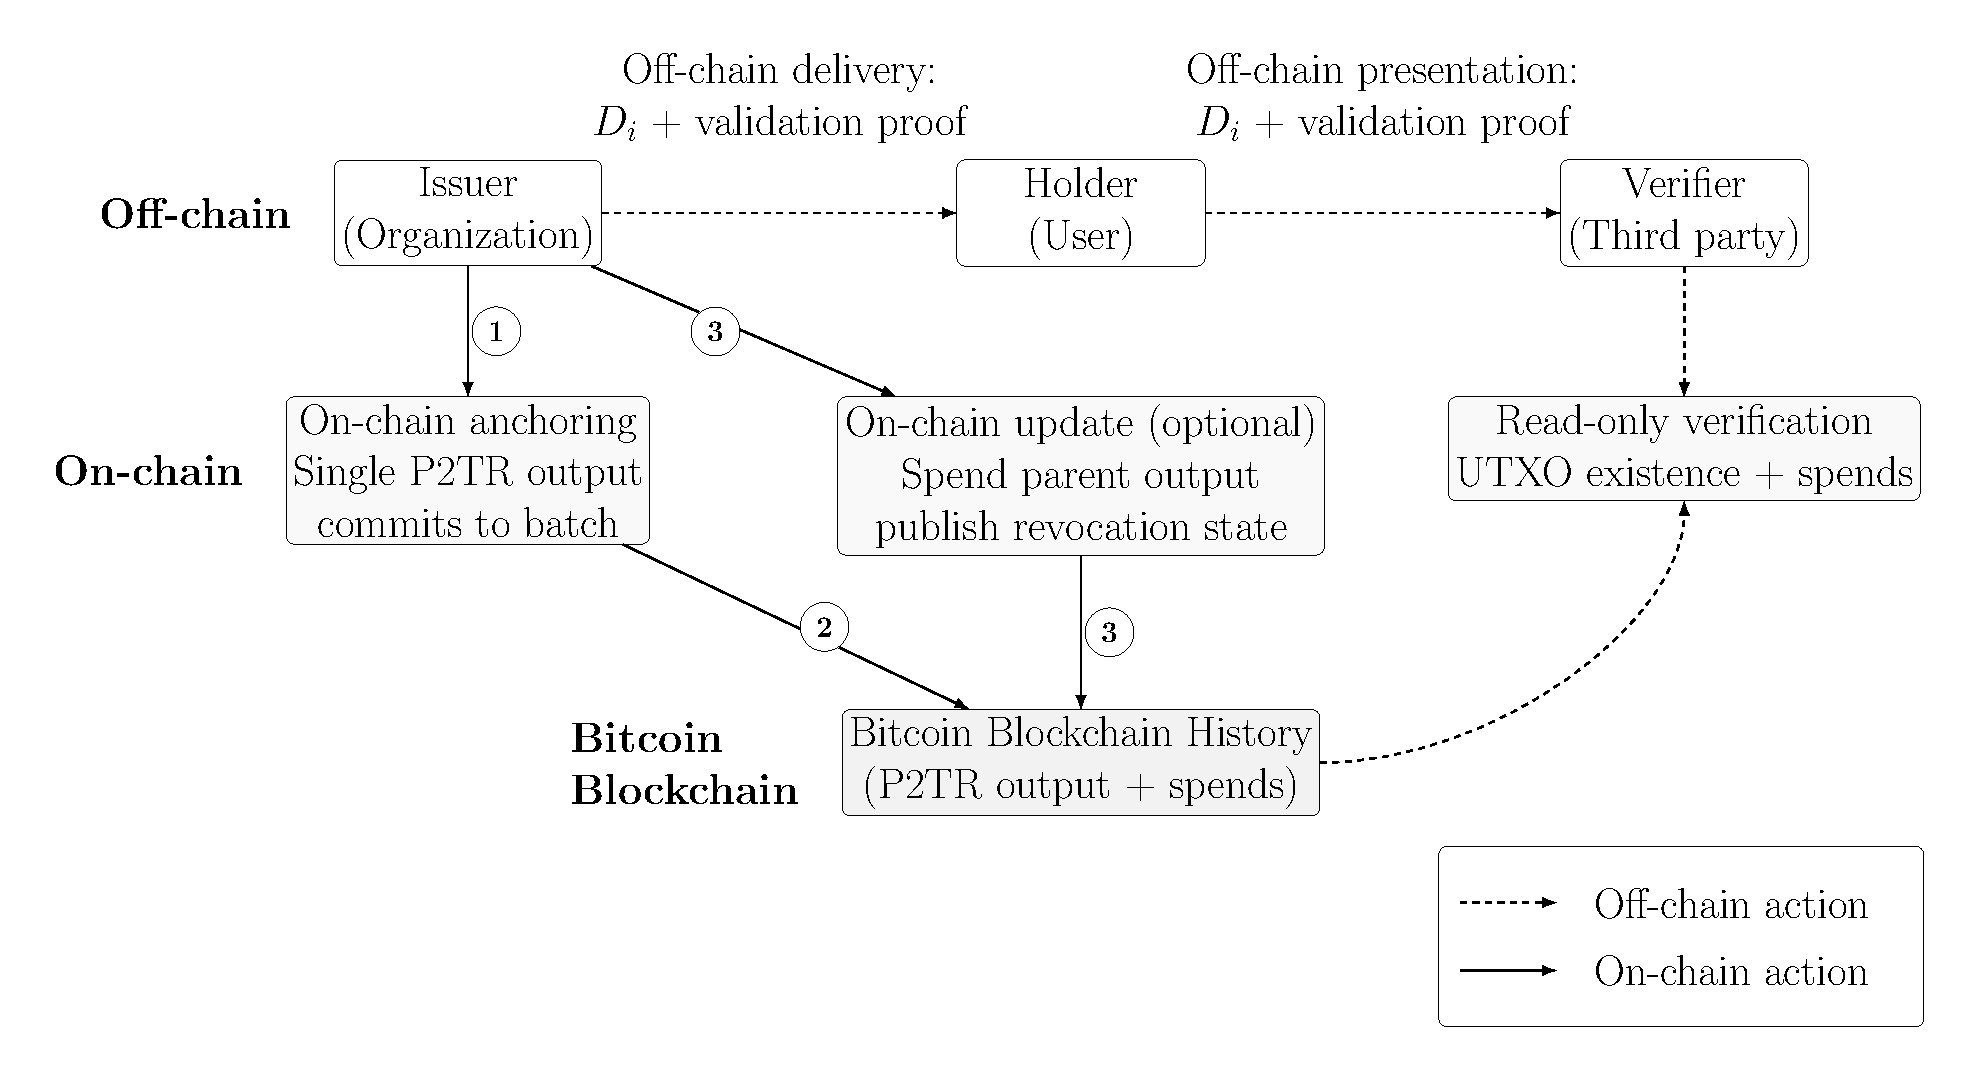
\includegraphics[width=\textwidth]{scheme_commit.pdf}
    \caption{System architecture and interaction flow of the proposed batch document verification protocol. 
(1) The issuer generates a batch commitment over a set of documents and anchors it on-chain by creating a single P2TR output. 
(2) Once confirmed, the commitment becomes part of the Bitcoin blockchain history. 
(3) Optionally, the issuer may later spend the committed output to publish an updated state, enabling revocation tracking. 
Off-chain, the issuer delivers each document $D_i$ together with its validation proof to the holder, who may later present them to a verifier. 
Verification is performed independently by checking the commitment and corresponding transactions in the Bitcoin blockchain, including UTXO existence and spending history, without requiring interaction with the issuer.}
    \label{fig:schemecommit}
\end{figure}



\subsection{Batch Commitment Construction}
\label{sec:createcommit}

Let us $\{D_i\}_{i=1}^{N}$ denote a batch of $N$ digital documents issued by a single organization.  The issuer controls a Schnorr signing key pair $(x_{\mathrm{iss}}, P_{\mathrm{iss}})$ used to guarantee authenticity. For each document $D_i$, the issuer computes:

\begin{equation}
h_i = H(D_i),
\label{eq:doc_hash}
\end{equation}

where $H(\cdot)$ is a collision-resistant hash function (e.g., SHA-256).

\paragraph{Script-leaf commitments.}

Each document is embedded into a Taproot script tree through a dedicated script leaf $S_i$.  Concretely, it $S_i$ encodes the tuple $(h_i, P_{\mathrm{iss}}, i)$, where it $i$ binds the commitment to its position within the batch. The corresponding Taproot leaf hash is computed following BIP341 as
\begin{equation}
\ell_i := H_{\text{TapLeaf}}(\textsf{leaf\_version} \parallel \textsf{len}(S_i) \parallel S_i).
\label{eq:tapleaf}
\end{equation}

The script is constructed such that script-path execution unconditionally fails.  
Consequently, spending through the script path is infeasible by construction, and the commitment is intended to be accessed exclusively via the key path.  Taproot script paths are therefore used purely as commitment carriers and are never intended to be revealed or executed.
Although the script paths are never intended to be executed, using Taproot script leaves provides a structured commitment mechanism compatible with the MAST framework.
This design preserves indistinguishability from standard P2TR outputs while allowing
future extensibility of script conditions without modifying the on-chain commitment.

\paragraph{Merkle aggregation.}

All leaf hashes $\{\ell_i\}_{i=1}^{N}$ are aggregated according to the Taproot Merkleization rules:

\begin{equation}
M = \textsf{TapMerkleRoot}(\ell_1, \ell_2, \ldots, \ell_N).
\label{eq:merkle_root}
\end{equation}

The Merkle root $M$ compactly commits to the entire batch of documents.

Figure~\ref{fig:merkle} illustrates the Merkle tree structure used in the proposed construction.  
Each leaf node corresponds to a Taproot script leaf embedding document-specific data, while internal nodes represent intermediate hashes computed according to the Taproot Merkleization rules.  
The root $M$ enables efficient per-document verification using a logarithmic-size Merkle authentication path without revealing information about other batch elements.

\begin{figure}[!h]
    \centering
    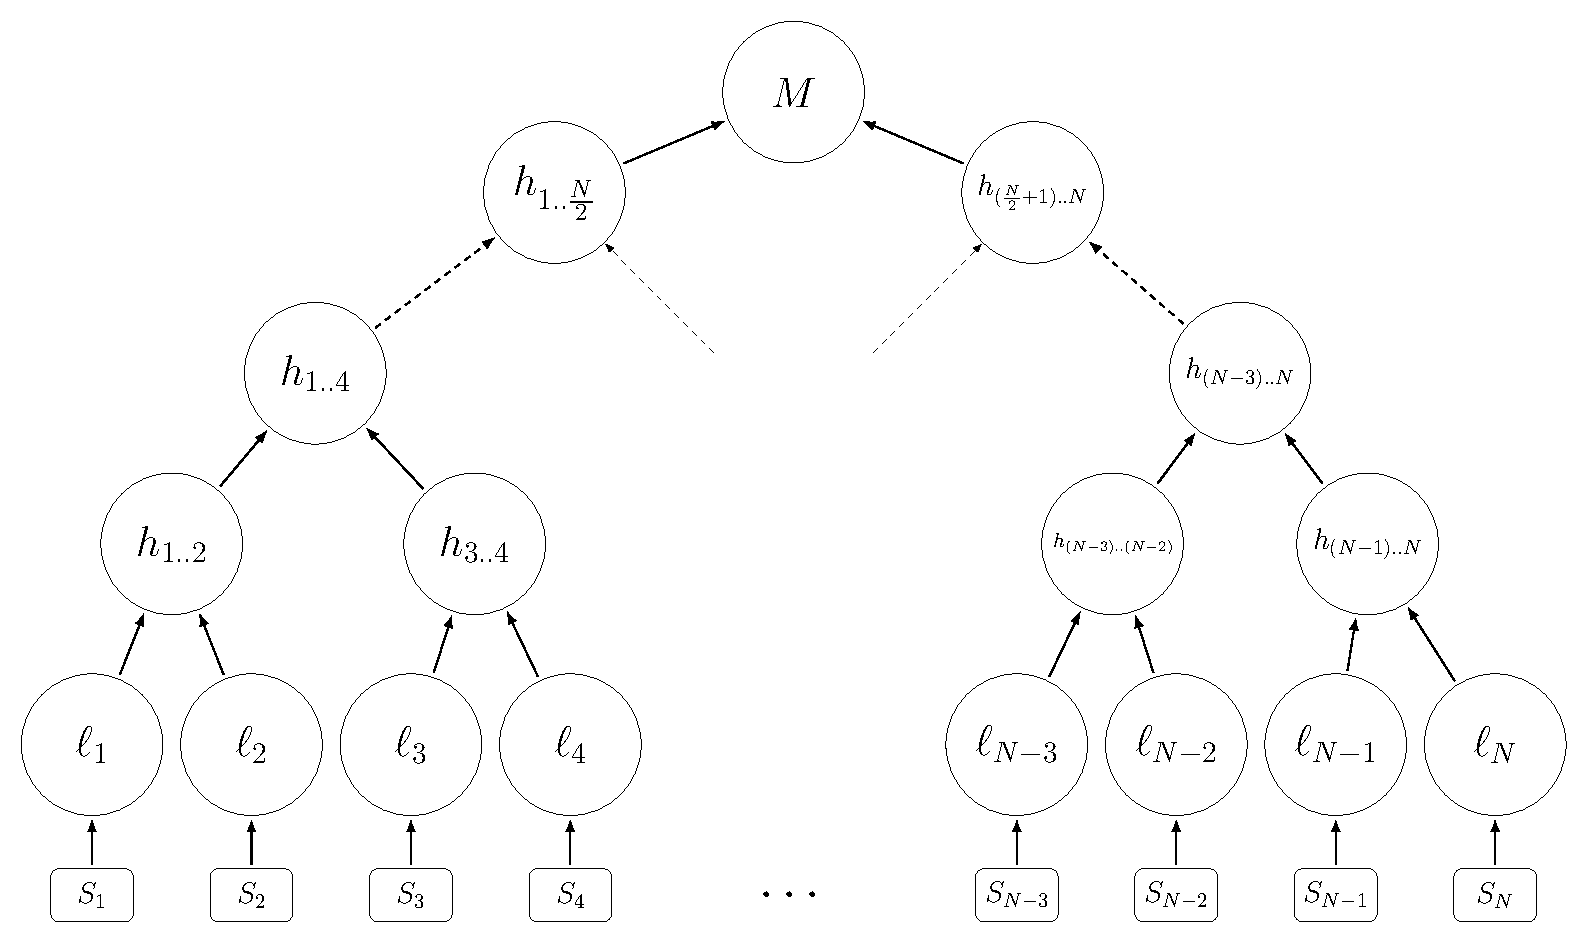
\includegraphics[width=0.8\textwidth]{merkle_tree.pdf}
    \caption{Merkle tree structure aggregating script-leaf commitments for a batch of $N$ documents.}
    \label{fig:merkle}
\end{figure}

\paragraph{Taproot output construction.}

Let $P_{\mathrm{int}}$ denote the internal Taproot public key controlled by the issuer.  
The Pay-to-Taproot output key is derived using the Taproot key-tweaking mechanism:

\begin{equation}
P_{\mathrm{out}} = P_{\mathrm{int}} + H_{\text{TapTweak}}(P_{\mathrm{int}} \parallel M)\,G,
\label{eq:taptweak}
\end{equation}

where $H_{\text{TapTweak}}(\cdot)$ is the tagged hash defined in BIP341 and $\parallel$ denotes concatenation.  
The resulting P2TR output $P_{\mathrm{out}}$ commits to $M$ while remaining indistinguishable from a standard key-path Taproot output.

\paragraph{On-chain anchoring.}

The issuer broadcasts a Bitcoin transaction $T_0$ that creates an output paying to $P_{\mathrm{out}}$.  
Once confirmed, the transaction identifier $\mathsf{txid}_0$ serves as the immutable reference for the batch commitment.


\subsection{Proof Generation}
\label{sec:proof_generation}

For each document $D_i$, the issuer generates a proof-of-validation object:

\begin{equation}
\pi_i := (\mathsf{txid}_0,\, i,\, P_{\mathrm{iss}},\, \sigma_i,\, \mathsf{path}_i),
\label{eq:proof}
\end{equation}

where:
\begin{itemize}
    \item $\mathsf{txid}_0$ is the anchoring transaction identifier,
    \item $i$ is the leaf index,
    \item $P_{\mathrm{iss}}$ is the issuer’s Schnorr public key,
    \item $\sigma_i$ is a Schnorr signature over a batch-bound message,
    \item $\mathsf{path}_i$ is the Merkle authentication path corresponding to $\ell_i$.
\end{itemize}

To prevent replay across batches, the issuer signs a message that binds the document to its anchoring transaction:

\begin{equation}
m_i := H_{\mathrm{sig}}(h_i \parallel i \parallel \mathsf{txid}_0),
\label{eq:signed_message}
\end{equation}

\begin{equation}
\sigma_i = \textsf{Sign}(x_{\mathrm{iss}}, m_i).
\label{eq:schnorr_signature}
\end{equation}

Algorithm~\ref{alg:p2tr_commit} summarizes the batch commitment and proof generation procedure executed by the issuer.

\begin{algorithm}[t]
\caption{Batch Commitment and Proof Generation}
\label{alg:p2tr_commit}
\begin{algorithmic}[1]
\Require Documents $\{D_i\}_{i=1}^{N}$, issuer key $(x_{\mathrm{iss}}, P_{\mathrm{iss}})$, internal key $P_{\mathrm{int}}$
\Ensure $P_{\mathrm{out}}$, proofs $\{\pi_i\}_{i=1}^{N}$

\For{$i \gets 1$ \textbf{to} $N$}
    \State $h_i \gets H(D_i)$
    \State Construct $S_i$ encoding $(h_i, P_{\mathrm{iss}}, i)$
    \State $\ell_i \gets H_{\text{TapLeaf}}(\textsf{leaf\_version} \parallel \textsf{len}(S_i) \parallel S_i)$
\EndFor

\State $M \gets \textsf{TapMerkleRoot}(\ell_1,\ldots,\ell_N)$
\State $t \gets H_{\text{TapTweak}}(P_{\mathrm{int}} \parallel M)$
\State $P_{\mathrm{out}} \gets P_{\mathrm{int}} + tG$
\State Broadcast $T_0$ creating output to $P_{\mathrm{out}}$

\For{$i \gets 1$ \textbf{to} $N$}
    \State $\mathsf{path}_i \gets \textsf{MerklePath}(i, \{\ell_j\})$
    \State $m_i \gets H_{\mathrm{sig}}(h_i \parallel i \parallel \mathsf{txid}_0)$
    \State $\sigma_i \gets \textsf{Sign}(x_{\mathrm{iss}}, m_i)$
    \State $\pi_i \gets (\mathsf{txid}_0, i, P_{\mathrm{iss}}, \sigma_i, \mathsf{path}_i)$
\EndFor

\State \Return $P_{\mathrm{out}}, \{\pi_i\}$
\end{algorithmic}
\end{algorithm}

\subsection{Verification Procedure}
\label{sec:verification_procedure}

Verification is performed entirely off-chain using the document $D_i$, the proof $\pi_i$, and read-only access to blockchain history. 
Algorithm~\ref{alg:verification} describes the verification procedure executed by the verifier. 
The process reconstructs the committed Merkle root, derives the Taproot output key, verifies the on-chain commitment, checks the issuer's Schnorr signature, and finally validates the revocation state associated with the document.

\begin{algorithm}[t]
\caption{Document Verification}
\label{alg:verification}
\begin{algorithmic}[1]
\Require $D_i$, $\pi_i$
\Ensure Accept or Reject

\State $h_i \gets H(D_i)$
\State Reconstruct $\ell_i$ and compute $M$ using $\mathsf{path}_i$
\State Derive $P_{\mathrm{out}}$ using Eq.~(\ref{eq:taptweak})
\State Verify that transaction $\mathsf{txid}_0$  contains an output paying to $P_{\mathrm{out}}$
\If{UTXO not found}
    \State \Return Reject
\EndIf

\State $m_i \gets H_{\mathrm{sig}}(h_i \parallel i \parallel \mathsf{txid}_0)$
\If{$\textsf{Verify}(P_{\mathrm{iss}}, m_i, \sigma_i) = \text{false}$}
    \State \Return Reject
\EndIf

\State Retrieve latest revocation bitmap $B_k$
\If{$B_k[i] = 1$}
    \State \Return Reject
\EndIf

\State \Return Accept
\end{algorithmic}
\end{algorithm}

Figure~\ref{fig:verification_flow} illustrates the verification workflow executed by the verifier. 

\begin{figure}[htbp]
\centering
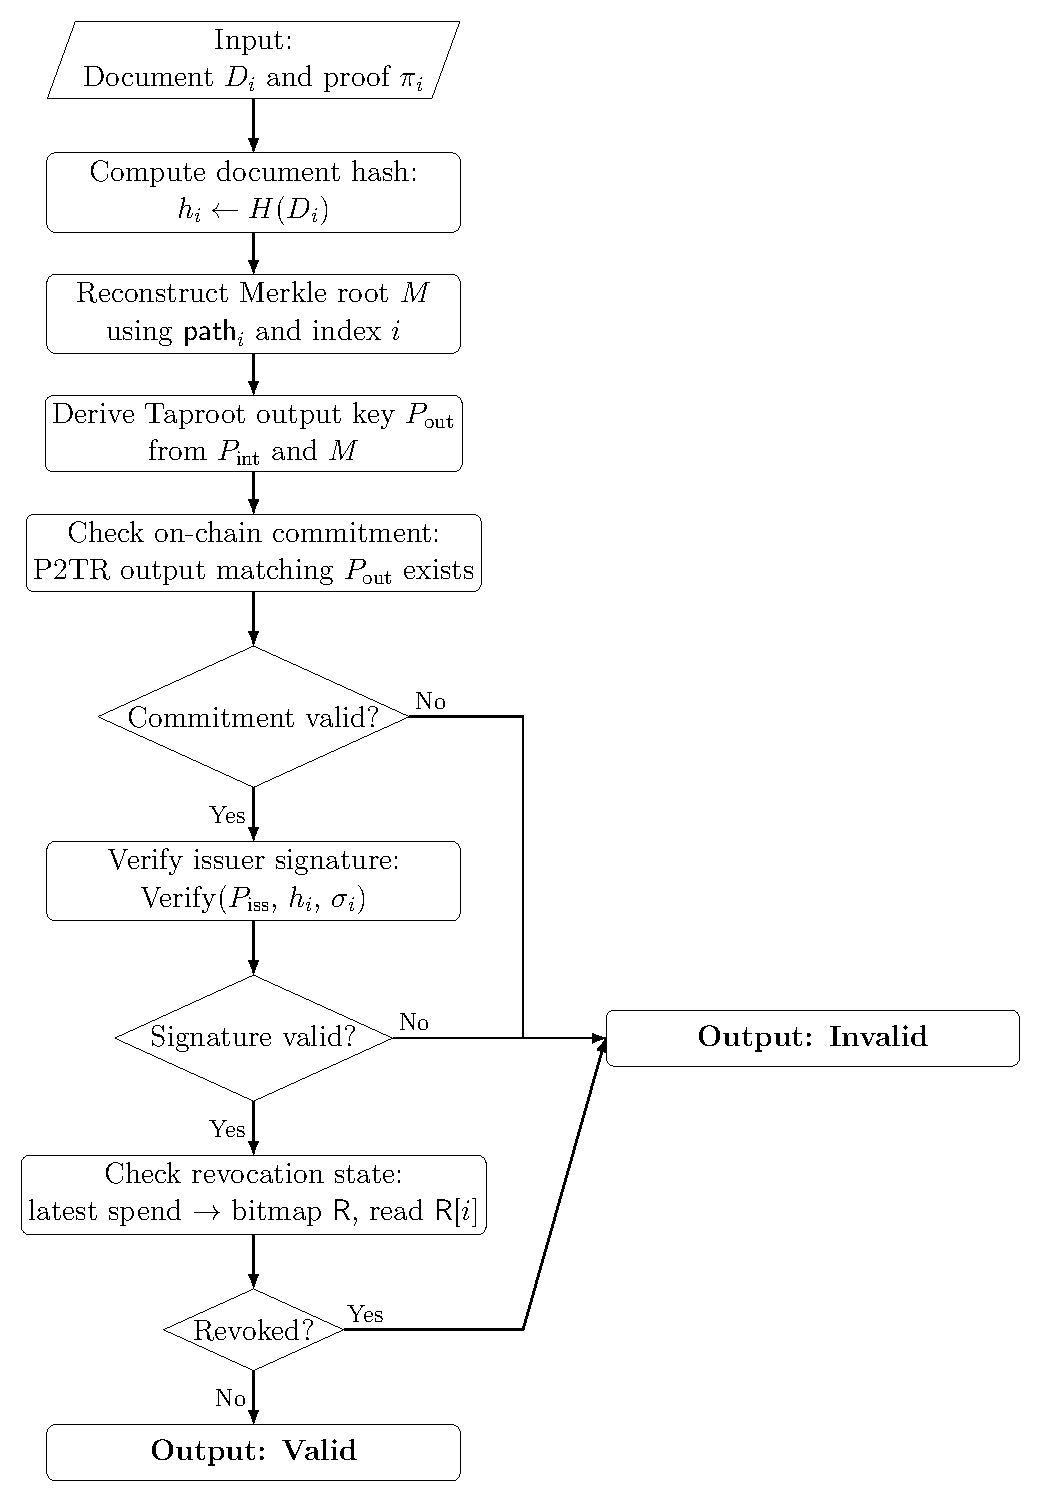
\includegraphics[width=.9\columnwidth]{verification.pdf}
\caption{Verification workflow for a document and its proof-of-validation.}
\label{fig:verification_flow}
\end{figure}

Given a document $D_i$ and its corresponding proof-of-validation $\pi_i$, the verifier first computes the document hash and reconstructs the Merkle root using the authentication path contained in the proof. 
From the reconstructed root and the internal Taproot key, the verifier derives the Taproot output key $P_{\mathrm{out}}$ and checks whether a corresponding P2TR output exists in the Bitcoin blockchain. 
If the commitment is valid, the verifier then checks the issuer's Schnorr signature bound to the document and the anchoring transaction. 
Finally, the verifier retrieves the most recent revocation bitmap and verifies that the corresponding index has not been marked as revoked. 
Only if all checks succeed is the document considered valid.



\subsection{Revocation Mechanism}
\label{sec:revocation}

Bitcoin immutability prevents modification of $T_0$.  Revocation is implemented through transaction chaining. Let us $T_k$ denote the $k$-th descendant transaction that spends the previous P2TR output via the key path and recreates an equivalent output committing to the same Merkle root $M$. Each update transaction $T_k$ includes an additional \texttt{OP\_RETURN} output encoding a revocation bitmap:

\begin{equation}
B_k \in \{0,1\}^N,
\end{equation}

where $B_k[i]=1$ indicates revocation of document $D_i$.

The size of $B_k$ is $|B_k| = N$ bits, implying an on-chain data cost of $\lceil N/8 \rceil$ bytes per revocation update.  
The economic impact of this linear growth is evaluated in Section~\ref{sec:evaluation}.
The valid revocation state corresponds to the bitmap included in the most recent confirmed descendant transaction in the canonical blockchain.


\subsection{Design Properties}

The proposed protocol satisfies the following security and functional properties:

\begin{enumerate}
    \item Document Integrity.
    Only documents included in the original batch commitment can produce a valid verification proof. 
    Any document outside the committed set cannot generate a valid Merkle authentication path consistent with the on-chain commitment.

    \item Issuer Authenticity. 
    The authenticity of issued documents is guaranteed through Schnorr signatures. 
    Security follows from the EUF-CMA  security of Schnorr signatures as specified in BIP340.

    \item Revocation Soundness. 
    Once a revocation update transaction is confirmed on-chain, any previously issued document marked as revoked can no longer be successfully verified as valid.

    \item Commitment Privacy. 
    Taproot ensures that unused script leaves remain hidden under the commitment structure. 
    As a result, observers cannot distinguish whether a transaction encodes a simple payment or a commitment to a complex verification structure.
\end{enumerate}

Formal security definitions and reduction arguments are presented in the following section.



\section{Security Definitions and Proof Sketch}
\label{sec:security}

This section formalizes the security guarantees of the proposed construction under standard cryptographic assumptions. We define the adversarial model, specify formal security properties, and provide reduction-based proof sketches demonstrating that any successful adversary would imply a break of underlying primitives.

\subsection{Adversarial Model}

We consider a probabilistic polynomial-time (PPT) adversary $\mathcal{A}$ interacting with the system after the anchoring transaction $T_0$ has been confirmed. The adversary is granted the following capabilities:

\begin{itemize}
    \item Access to all public blockchain data, including $T_0$ and its descendant transactions.
    \item Access to any document $D_i$ and its corresponding proof-of-validation $\pi_i$.
    \item The ability to generate arbitrary candidate documents $D^*$ and arbitrary forged proofs $\pi^*$.
\end{itemize}

The adversary does not control a majority of the global hash rate and therefore cannot rewrite confirmed blockchain history. We assume standard Nakamoto consensus security under the honest-majority assumption. Cryptographic primitives are modeled under standard security assumptions:

\begin{itemize}
    \item The hash function $H(\cdot)$ is collision resistant.
    \item Schnorr signatures are EUF-CMA secure under BIP340.
\end{itemize}

\textbf{Definition 1 (Valid Document).}  
A document $D_i$ with proof $\pi_i = (\mathsf{txid}_0, i, P_{\mathrm{iss}}, \sigma_i, \mathsf{path}_i)$ is considered valid if and only if:

\begin{enumerate}
    \item $h_i = H(D_i)$ reconstructs a leaf $\ell_i$ consistent with the Merkle root $M$ using $\mathsf{path}_i$;
    \item the derived $P_{\mathrm{out}}$ corresponds to a confirmed UTXO in transaction $\mathsf{txid}_0$;
    \item $\sigma_i$ verifies under $P_{\mathrm{iss}}$ for message 
    $m_i = H_{\mathrm{sig}}(h_i \parallel i \parallel \mathsf{txid}_0)$;
    \item the most recent revocation bitmap $B_k$ satisfies $B_k[i] = 0$.
\end{enumerate}


\textbf{Definition 2 (Correctness).}  
If the issuer follows the protocol honestly and $D_i$ has not been revoked, then the probability that the verification algorithm rejects $(D_i, \pi_i)$ is negligible.

\subsection{Security Assumptions}

The security of the proposed construction relies on several standard cryptographic and system-level assumptions commonly adopted in blockchain-based protocols.

First, the hash function $H(\cdot)$ instantiated with SHA-256 is assumed to be collision resistant. This property ensures that an adversary cannot construct two distinct inputs producing the same hash value, which guarantees the binding property of document commitments and the integrity of the Merkle tree structure.

Second, the Schnorr signature scheme defined in BIP340 is assumed to be EUF-CMA based on the hardness of the discrete logarithm problem in the secp256k1 elliptic curve group. Under this assumption, no adversary can generate a valid signature under the issuer's public key $P_{\mathrm{iss}}$ without knowledge of the corresponding private key $x_{\mathrm{iss}}$.

Finally, the security of the blockchain anchoring mechanism relies on the honest-majority assumption underlying Nakamoto consensus. Specifically, we assume that no adversary controls a majority of the global mining hash power, preventing modification of confirmed blockchain history and ensuring the immutability of the anchoring transaction $T_0$ and its descendant revocation transactions.
Under these assumptions, the proposed construction achieves scalable, revocable, and authenticity-preserving document verification anchored to the Bitcoin blockchain.

\subsection{Security Properties}

This analysis focuses on three fundamental properties: batch integrity, issuer authenticity, and revocation soundness. Additionally, we discuss the impact of the issuer's private key compromise and loss on the security guarantees of the system.

Integrity ensures that only documents originally included in the committed batch can be successfully verified.

\textbf{Definition 3 (Batch Integrity).}  
The construction satisfies batch integrity if no probabilistic polynomial-time (PPT) adversary $\mathcal{A}$ can produce a pair $(D^*, \pi^*)$ such that $D^*$ is not included in the original batch committed in transaction $T_0$, and the verification algorithm accepts $(D^*, \pi^*)$ with nonnegligible probability.

Intuitively, this property follows from the collision resistance of the hash function $H(\cdot)$ together with the binding property of the Merkle commitment rooted at $M$. Any successful forgery would require either constructing a second preimage for $H(\cdot)$ or producing a valid Merkle authentication path inconsistent with the committed root.

Authenticity guarantees that accepted proofs originate from the legitimate issuer controlling the signing key associated with $P_{\mathrm{iss}}$.

\textbf{Definition 4 (Authenticity).}  
The scheme satisfies issuer authenticity if no PPT adversary can produce a valid proof $\pi^*$ containing a signature $\sigma^*$ that verifies under $P_{\mathrm{iss}}$ for a message that was not signed by the legitimate issuer, except with negligible probability.

This property follows from the existential unforgeability under chosen-message attack (EUF-CMA) security of Schnorr signatures as specified in BIP340.

Revocation soundness ensures that documents explicitly marked as revoked cannot be successfully verified.

\textbf{Definition 5 (Revocation Soundness).}  
The scheme satisfies revocation soundness if, once a revocation bitmap $B_k$ is confirmed on-chain with $B_k[i] = 1$, no PPT adversary can produce a proof $\pi_i$ that is accepted by the verification algorithm for document $D_i$.

This property follows from the requirement that the verification algorithm always evaluates the most recent confirmed revocation bitmap associated with the commitment chain originating from $T_0$.

Finally, we consider the implications of issuer private key compromise and key loss for the security of the system. If the issuer's Schnorr private key $x_{\mathrm{iss}}$ is compromised after issuance, previously anchored documents remain cryptographically intact. Integrity depends only on the collision resistance of the committed hash values and the immutability of the anchoring transaction $T_0$. However, authenticity of future documents can no longer be guaranteed under the compromised key.

In contrast, if the private key is irreversibly lost, the issuer can no longer generate valid signatures for newly issued documents. Nevertheless, previously issued and anchored documents remain verifiable because verification requires only the public key $P_{\mathrm{iss}}$ and the commitment recorded in $T_0$. Therefore, key loss affects only the ability to issue new documents, while previously anchored documents remain valid. This separation between commitment integrity and signing capability is a direct consequence of anchoring document commitments independently from the issuer's signing state.

\subsection{Reduction Arguments}

We now provide proof sketches showing that any successful adversary against the proposed construction would imply a break of the underlying cryptographic assumptions.

\textbf{\\Theorem 1 (Integrity).}  
If an adversary succeeds in the batch integrity game with non-negligible probability, then one can construct an algorithm that either finds a collision in the hash function $H(\cdot)$ or produces a Merkle authentication path inconsistent with the committed root $M$.

\begin{proof}
A successful adversary must produce a pair $(D^*, \pi^*)$ that is accepted by the verification algorithm while $D^*$ was not included in the original batch committed in $T_0$. Acceptance requires reconstruction of a Merkle authentication path leading to the root $M$. Since the Taproot output key $P_{\mathrm{out}}$ is deterministically derived from $M$, the reconstructed root must equal the committed value. Therefore, the adversary must either construct two distinct inputs that hash to the same leaf value or produce an alternative authentication path yielding the same Merkle root. Both cases reduce to violating the collision resistance of $H(\cdot)$.
\end{proof}

\textbf{\\Theorem 2 (Authenticity).}  
If an adversary produces a valid proof containing a forged signature under the public key $P_{\mathrm{iss}}$, then one can construct an algorithm that breaks the existential unforgeability under chosen-message attack (EUF-CMA) security of Schnorr signatures.

 \begin{proof} 

A proof $\pi_i$ is accepted only if the signature $\sigma_i$ verifies under $P_{\mathrm{iss}}$ for the message $m_i = H_{\mathrm{sig}}(h_i \parallel i \parallel \mathsf{txid}_0)$. Since the message binds the document hash, its batch position, and the anchoring transaction identifier, producing a valid signature $\sigma^*$ without knowledge of the secret key $x_{\mathrm{iss}}$ constitutes a direct Schnorr forgery. Consequently, any adversary capable of producing such a proof can be used to break the EUF-CMA security of the Schnorr signature scheme defined in BIP340.
\end{proof} 

\textbf{\\Theorem 3 (Revocation Soundness).}  
Assuming the immutability of confirmed blockchain history under Nakamoto consensus, revocation soundness holds.
\begin{proof} 
Once a revocation bitmap $B_k$ is confirmed in a descendant transaction of $T_0$ with $B_k[i] = 1$, the verification algorithm deterministically rejects document $D_i$. A successful adversary would therefore need to either alter the confirmed revocation bitmap or rewrite blockchain history to remove the revocation transaction. Both scenarios contradict the honest-majority assumption underlying the security of Nakamoto consensus. 
\end{proof}

\subsection{Extended Attack Analysis}

Beyond the formal cryptographic reductions presented previously, we consider several additional attack vectors relevant to practical deployment of the proposed construction. These scenarios do not violate the underlying security assumptions but may arise in adversarial environments interacting with the protocol.

Replay attacks across distinct document batches are prevented through explicit binding of signatures to the anchoring transaction identifier. In particular, each verification message includes the value $\mathsf{txid}_0$, ensuring that a signature $\sigma_i$ produced for one batch commitment cannot be reused in another commitment context. Any attempt to reuse $\sigma_i$ across batches would therefore fail during verification because the reconstructed message would differ.

Selective disclosure attacks are mitigated through the use of Merkle authentication paths. A verifier receives only the authentication path $\mathsf{path}_i$ corresponding to the document being verified, which reveals no information about other documents contained in the batch. Consequently, the protocol enables per-document verification while preserving the privacy of unrelated batch elements.

Key compromise scenarios are also considered. If the issuer's private signing key $x_{\mathrm{iss}}$ is compromised after document issuance, previously anchored documents remain cryptographically valid. Their integrity relies solely on the collision resistance of the committed hash values and the immutability of the anchoring transaction $T_0$. However, authenticity of future document issuances can no longer be guaranteed under the compromised key. This limitation is inherent to any public-key infrastructure and does not affect the security of already anchored commitments.

Finally, denial-of-service considerations are limited to infrastructure availability rather than protocol correctness. The verification procedure is stateless and requires only read-only access to blockchain data. As a result, denial-of-service attacks can only affect the availability of blockchain nodes or network connectivity and cannot compromise the integrity of the anchored commitments.



\section{Comparative Evaluation}
\label{sec:evaluation}

This section evaluates the scalability and cost characteristics of the proposed construction as a function of the batch size $N$. 
The goal of this evaluation is to quantify how the protocol behaves when the number of committed documents increases. 
In particular, we analyze four metrics that directly affect the practicality of the system: the size of the anchoring transaction, the size of the verification proof, the computational cost of verification, and the cost of revocation updates.

All on-chain costs are expressed in virtual bytes (vB), which represent the canonical fee metric used in Bitcoin. 
Transaction fees are determined by the mempool fee rate (sat/vB), which fluctuates depending on network congestion. Because this parameter varies over time and is external to protocol design, reporting costs in satoshis or USD would introduce non-reproducible variability. 
For this reason, all transaction costs are expressed purely in vB, defined as

\begin{equation}
\mathrm{vB} = \frac{\mathrm{weight\ units}}{4},
\end{equation}

following Bitcoin's weight accounting rules. 
Given a mempool fee rate $\rho$ (sat/vB), the resulting transaction fee would be

\begin{equation}
\mathrm{fee} = \rho \cdot \mathrm{vB},
\end{equation}

but $\rho$ is treated as an external parameter and is therefore not fixed in this analysis.

The evaluation focuses on four quantities that determine the scalability of the protocol:

\begin{itemize}
\item the issuance transaction size $\mathrm{vB}(T_0)$,
\item the proof size $|\pi_i|$,
\item the verification complexity $t_{\mathrm{ver}}(N)$,
\item the revocation update transaction size $\mathrm{vB}(T_k)$.
\end{itemize}

The anchoring transaction $T_0$ embeds the Merkle root inside the Taproot output key. 
Because the Merkle root is a fixed-size value independent of the number of documents in the batch, the size of the issuance transaction does not depend on $N$. 
The transaction size can therefore be expressed as

\begin{equation}
\mathrm{vB}(T_0) = C_{\mathrm{iss}},
\end{equation}

where $C_{\mathrm{iss}}$ denotes the constant size of the transaction template containing a standard P2TR output. 
This property implies that the issuance cost remains constant regardless of the number of committed documents.

The proof size grows logarithmically with the batch size due to the Merkle authentication path. 
Let $d = \lceil \log_2 N \rceil$ denote the depth of the Merkle tree. 
Each proof contains $d$ sibling hashes (32 bytes each), one Schnorr signature (64 bytes), and several fixed-size metadata fields including the transaction identifier, index, and issuer public key. 
The resulting proof size can therefore be written as

\begin{equation}
|\pi_i| = C_{\mathrm{proof}} + 32\lceil\log_2 N\rceil.
\label{eq12}
\end{equation}

Figure~\ref{fig:proofsize} illustrates the growth of the proof size as a function of the batch size $N$.  The results confirm the logarithmic behavior predicted by Eq.~(\ref{eq12}), showing that proof size increases slowly even for large batches.  This property enables scalable document verification while maintaining compact validation proofs.


Verification requires reconstructing the Merkle root and validating the issuer signature. 
Consequently, the computational cost consists of $\lceil\log_2 N\rceil$ hash evaluations and a single Schnorr signature verification. 
The verification time can therefore be modeled as

\begin{equation}
t_{\mathrm{ver}}(N) = a \cdot \lceil\log_2 N\rceil + b,
\end{equation}

where the constants $a$ and $b$ depend on the implementation environment. Figure~\ref{fig:verificationtime} shows the verification time as the batch size increases. 
The parameters $a = 0.02$ ms and $b = 0.10$ ms were obtained from experimental measurements of SHA-256 hashing and Schnorr signature verification on a standard workstation. The results confirm the logarithmic verification complexity predicted by Eq.~(13), demonstrating that verification remains efficient even for large document batches.

Revocation is implemented through a bitmap published in the revocation transaction. 
If the batch contains $N$ documents, the bitmap requires

\begin{equation}
|B_k| = \left\lceil \frac{N}{8} \right\rceil \text{ bytes}.
\end{equation}

The total size of the revocation transaction is therefore

\begin{equation}
\mathrm{vB}(T_k) = C_{\mathrm{rev}} + \left\lceil \frac{N}{8} \right\rceil,
\end{equation}

where $C_{\mathrm{rev}}$ represents the constant overhead of the transaction template. For a fixed batch size $N$, subsequent revocation updates do not increase this value because each update republishes a bitmap of identical length. Figure~\ref{fig:revocationcost} illustrates the revocation transaction size as the batch size increases. 
The results confirm the linear growth predicted by Eq.~(15), since the revocation bitmap requires $\lceil N/8 \rceil$ bytes to encode the state of $N$ documents.


Table~\ref{tab:scaling_summary} summarizes the scalability properties of the proposed construction using the metrics described above. 
The table highlights how each component of the protocol behaves as the batch size increases. 
In particular, the issuance transaction size remains constant in vB, reflecting the $\mathcal{O}(1)$ anchoring cost achieved by committing the entire batch through a single Taproot output. 
In contrast, the proof size and verification complexity grow logarithmically with $N$, which is expected for Merkle-based constructions. 
Revocation updates grow linearly with the batch size because the bitmap encoding requires $\mathcal{O}(N)$ space.

The concrete instantiations for $2^{10}$, $2^{14}$, and $2^{16}$ documents demonstrate that proof growth remains moderate even for large batches, while the issuance cost remains constant and the verification procedure requires only a small number of hash operations together with a single signature verification.

\begin{figure}[htbp]
\centering
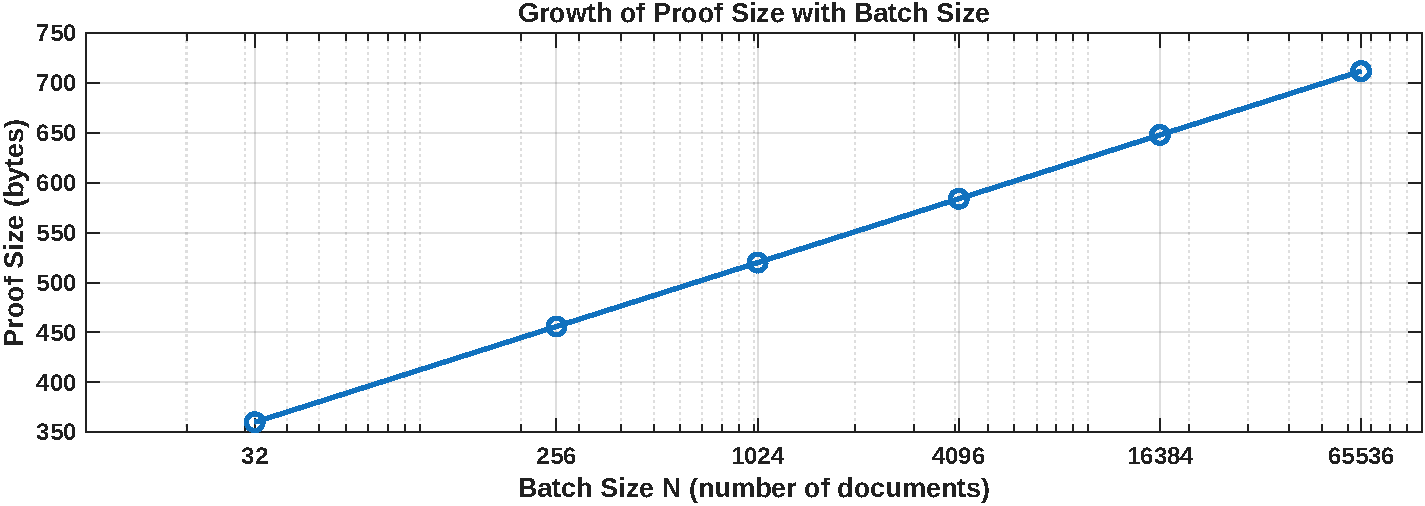
\includegraphics[width=0.75\columnwidth]{Figure_1.pdf}
\caption{Proof size growth as a function of batch size $N$}
\label{fig:proofsize}
\end{figure}



\begin{figure}[htbp]
\centering
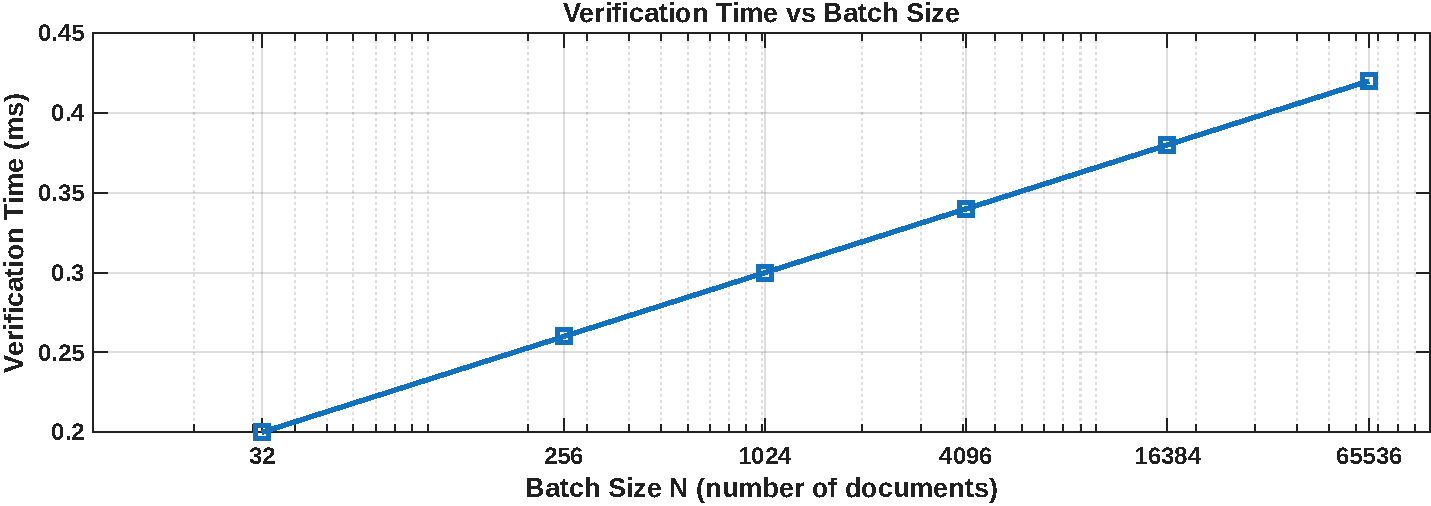
\includegraphics[width=0.75\columnwidth]{Figure_2.pdf}
\caption{Verification time as a function of batch size $N$}
\label{fig:verificationtime}
\end{figure}

\begin{figure}[htbp]
\centering
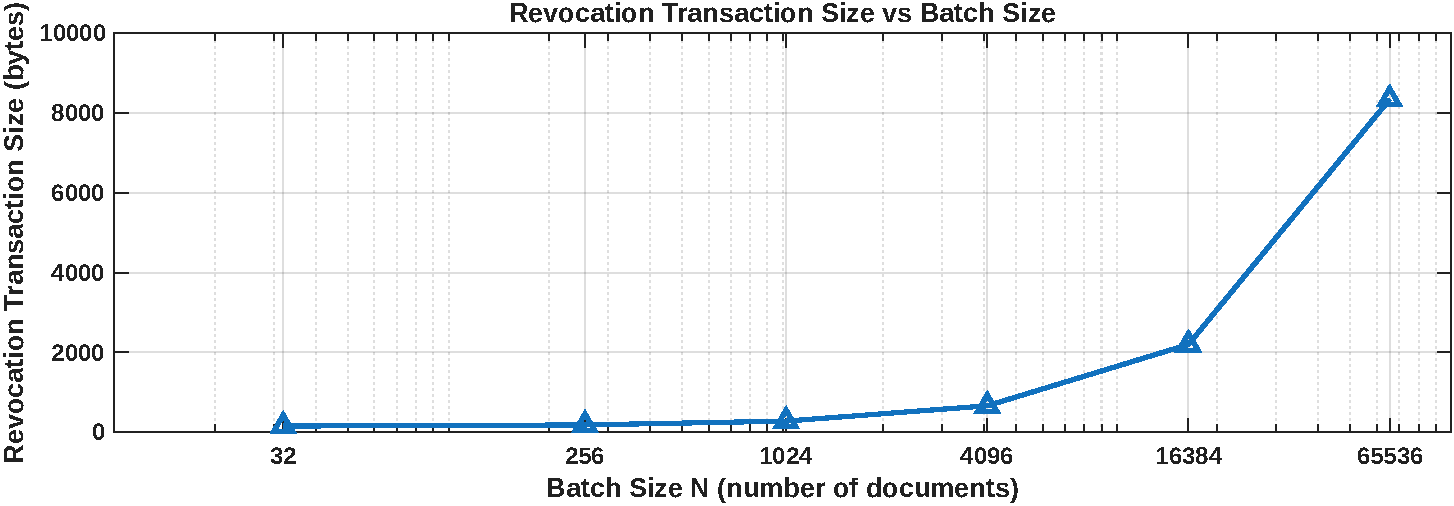
\includegraphics[width=0.75\columnwidth]{Figure_3.pdf}
\caption{Revocation transaction size as a function of batch size $N$}
\label{fig:revocationcost}
\end{figure}

\begin{table}[t]
\caption{Scalability of the proposed construction as a function of batch size $N$. On-chain costs are reported exclusively in virtual bytes (vB).}
\label{tab:scaling_summary}
\centering
\small
\renewcommand{\arraystretch}{1.2}

\begin{adjustbox}{max width=\linewidth}
\begin{tabular}{
>{\centering\arraybackslash}m{2.8cm}
c
c
>{\centering\arraybackslash}m{4cm}
>{\centering\arraybackslash}m{3.2cm}
}
\toprule
\textbf{Batch size $N$} &
\shortstack{\textbf{Issuance size}\\$\mathrm{vB}(T_0)$} &
\shortstack{\textbf{Proof size}\\$|\pi_i|$ (bytes)} &
\textbf{Verification complexity} &
\shortstack{\textbf{Revocation size}\\$\mathrm{vB}(T_k)$} \\
\midrule

$\mathcal{O}(N)$ &
$\mathcal{O}(1)$ &
$\mathcal{O}(\log N)$ &
$\mathcal{O}(\log N)$ &
$\mathcal{O}(N)$ \\
\midrule

$2^{10}$ (1,024) &
$C_{\mathrm{iss}}$ &
$C_{\mathrm{proof}} + 320$ &
$\sim 10$ hash ops + 1 sig &
$C_{\mathrm{rev}} + 128$ \\

$2^{14}$ (16,384) &
$C_{\mathrm{iss}}$ &
$C_{\mathrm{proof}} + 448$ &
$\sim 14$ hash ops + 1 sig &
$C_{\mathrm{rev}} + 2{,}048$ \\

$2^{16}$ (65,536) &
$C_{\mathrm{iss}}$ &
$C_{\mathrm{proof}} + 512$ &
$\sim 16$ hash ops + 1 sig &
$C_{\mathrm{rev}} + 8{,}192$ \\

\bottomrule
\end{tabular}
\end{adjustbox}

\end{table}



Another comparison considers representative blockchain-based document anchoring approaches in order to contextualize the proposed construction. 
Traditional anchoring techniques typically embed document hashes directly in Bitcoin transactions using mechanisms such as \texttt{OP\_RETURN}. 
While simple, this approach introduces a linear on-chain footprint because each document requires an individual commitment.

Merkle-based anchoring systems improve scalability by aggregating document hashes into a Merkle tree and anchoring only the root hash on-chain. 
This reduces the issuance cost to $\mathcal{O}(1)$ while preserving efficient per-document verification through logarithmic Merkle proofs. 
However, many existing systems do not natively support issuer authentication or explicit revocation mechanisms.

The proposed protocol preserves the scalability advantages of Merkle-based anchoring while integrating issuer authentication and revocation support through a Taproot-native construction. 
Table~\ref{tab:approach_comparison} provides a high-level comparison of representative Bitcoin document anchoring approaches, highlighting their scalability characteristics and support for authentication and revocation.

\begin{table}[t]
\centering
\caption{High-level comparison of representative Bitcoin document anchoring approaches.}
\label{tab:approach_comparison}
\small
\renewcommand{\arraystretch}{1.2}

\begin{adjustbox}{max width=\linewidth}
\begin{tabular}{
>{\raggedright\arraybackslash}m{4.5cm}
c c c c
}
\toprule
\textbf{Approach} &
\textbf{Issuance Cost} &
\textbf{Verification} &
\textbf{Revocation} &
\textbf{Authentication} \\
\midrule

\texttt{OP\_RETURN} Anchoring &
$\mathcal{O}(N)$ &
$\mathcal{O}(1)$ &
No &
No \\

Merkle Anchoring (e.g., OpenTimestamps) &
$\mathcal{O}(1)$ &
$\mathcal{O}(\log N)$ &
No &
No \\

Proposed Protocol &
$\mathcal{O}(1)$ &
$\mathcal{O}(\log N)$ &
Yes &
Yes \\

\bottomrule
\end{tabular}
\end{adjustbox}

\end{table}

This section discusses the broader implications of the proposed protocol, including its security and privacy guarantees, operational trade-offs, and deployment considerations. The analysis also highlights practical limitations and outlines directions for future research.

\subsection{Security Implications}

The security of the proposed construction relies on three standard assumptions: 
(i) collision resistance of the hash function $H(\cdot)$ (e.g., SHA-256), 
(ii) existential unforgeability under chosen-message attacks (EUF-CMA) of Schnorr signatures defined in BIP340, 
and (iii) the honest-majority security of Nakamoto consensus.
Under these assumptions, the protocol guarantees batch integrity, issuer authenticity, and revocation soundness as defined in Section~\ref{sec:security}. 
Once the anchoring transaction $T_0$ is confirmed, document inclusion becomes immutable unless an adversary can either violate the collision resistance of $H(\cdot)$ or rewrite confirmed blockchain history.

Key management for the issuer keys $P_{\mathrm{int}}$ and $x_{\mathrm{iss}}$ remains orthogonal to the protocol design. 
However, the linearity of Schnorr signatures enables straightforward integration of threshold or multisignature constructions without modifying the verification algorithm. 
This property is particularly useful for institutional deployments where distributed authorization or multi-party approval is required.

\subsection{Privacy Considerations}

The protocol provides selective disclosure at the batch level through the use of Merkle authentication paths. 
During verification, only the authentication path corresponding to the verified document is revealed, while other leaves in the batch remain hidden. 
As a result, verification does not expose unrelated documents or their contents.

Nevertheless, all documents anchored in the same transaction remain publicly linkable through the transaction identifier $\mathsf{txid}_0$. 
Consequently, the protocol preserves confidentiality of document contents and unrelated batch elements, but does not provide unlinkability between documents issued within the same batch.



\subsection{Scalability Trade-offs}

The primary scalability trade-off arises from the revocation bitmap encoding used by the protocol. 
As analyzed in Section~\ref{sec:evaluation}, the size of revocation transactions grows linearly with the batch size $N$, since the bitmap requires $\lceil N/8 \rceil$ bytes.
Consequently, the protocol exhibits an asymmetric scalability profile: issuance cost remains constant and verification complexity grows logarithmically, while revocation updates introduce linear on-chain growth. 
For a fixed batch size $N$, subsequent revocation updates do not increase the bitmap length, meaning that each additional revocation update incurs constant marginal cost once the batch size is fixed.

In practice, relay policy limits on \texttt{OP\_RETURN} payload size impose an upper bound on feasible batch sizes when revocation support is required. 
These limits must therefore be considered when selecting batch sizes for operational deployments.
Alternative revocation encodings could further improve asymptotic scalability.
For example, Merkle-based accumulators or sparse Merkle trees could replace the
bitmap representation while preserving logarithmic verification complexity.
Such approaches represent an interesting direction for future work.
\vspace{-0.3cm}
\subsection{Deployment Considerations}

The proposed construction is fully compatible with existing Bitcoin infrastructure and requires no modifications to the underlying protocol. 
Verification is entirely read-only and does not require interaction with the issuer once the proof-of-validation has been distributed.

Operational deployments should nevertheless consider several organizational factors, including key rotation policies, long-term archival storage of proofs, and the selection of batch sizes relative to expected revocation frequency. 
Careful coordination between issuance policies and revocation requirements is necessary to maintain long-term operational efficiency.

Future work includes empirical benchmarking of issuance and revocation costs under real mainnet conditions, exploration of alternative revocation encodings such as Merkle accumulators, and adaptive batch segmentation strategies that balance issuance efficiency with revocation overhead.

\subsection{Institutional Key Governance}

To mitigate risks associated with single-key control, the issuer key $P_{\mathrm{iss}}$ can be instantiated as an aggregated MuSig2 public key derived from multiple institutional actors.
For example, a university deployment may construct a three-party aggregated key composed of the Academic Director of the department, the Head of Information Systems, and the Dean of the faculty. 
Using MuSig2 key aggregation, these actors jointly generate a single aggregated public key $P_{\mathrm{agg}}$ that replaces $P_{\mathrm{iss}}$ in the protocol.

Document signatures are then generated through interactive threshold signing while keeping individual private key shares confidential. 
This approach eliminates single points of failure, prevents unilateral document issuance, and improves institutional accountability through distributed authorization.
Importantly, MuSig2 preserves the single public key abstraction of Schnorr signatures. 
As a result, verifiers continue to validate a single signature under $P_{\mathrm{agg}}$, meaning that the verification procedure remains unchanged while operational security is strengthened.
This design prevents unilateral document issuance and reduces the risk
associated with single-key compromise in institutional deployments.

\subsection{Performance Outlook}

Overall, the protocol achieves constant-size issuance cost, logarithmic verification complexity $O(\log N)$, and linear revocation update size $O(N)$. 
This asymmetric scaling profile shifts long-term operational costs toward revocation management while preserving efficient verification even for very large document batches.



%%%%%%%%%%%%%%%%%%%%%%%%%%%%%%%%%%%%%%%%%%%%%%%%%%%%%%%%%%%%%%%%%%%%%%%%%%%%%%%%%%%%%%%%%%%%%%%%%%%%%%%%%%%%%%%%%%%%%%%%%%%%%%%%%%%%%%%%%%%%%%%%%%%%%


\section{Conclusion and Future Work}
\label{sec_Conclusion}

This paper presents a Taproot-based document verification protocol that enables scalable batch commitments, issuer authenticity guarantees, and explicit revocation support using only standardized Bitcoin primitives. Unlike prior Bitcoin-based anchoring approaches that focus solely on integrity, the proposed construction integrates batch aggregation, signature binding, and lifecycle state management within a unified Taproot-native design. The protocol achieves constant-size issuance cost, logarithmic verification complexity, and linear revocation update cost with respect to batch size. By leveraging Schnorr signatures and Merkleized script commitments, the construction preserves privacy of non-related batch elements and avoids on-chain disclosure of document data. 

Revocation is implemented through publicly auditable state transitions without invalidating prior commitments. Importantly, the results demonstrate that expressive smart contract execution is not required to implement scalable and revocable certification systems at the Bitcoin base layer. 
Taproot provides sufficient cryptographic structure to support advanced non-monetary applications while preserving Bitcoin’s minimal execution model. 

Future research directions include alternative revocation encodings with improved asymptotic behavior, privacy-enhancing verification mechanisms, and long-term archival strategies for proof persistence. Overall, the findings indicate that Taproot significantly expands the design space for decentralized verification systems on Bitcoin, enabling practical, privacy-preserving certification architectures that operate without trusted intermediaries.
Future work may also explore privacy-enhancing extensions such as zero-knowledge proofs capable of hiding Merkle path positions or issuer metadata. 
Such approaches not only improve unlinkability properties, they would also introduce additional computational overhead and implementation complexity.

\section*{Acknowledgment}
The author would like to thank King Fahd University of Petroleum and Minerals, Dhahran, Saudi Arabia, for supporting this research. 
Authors would like to acknowledge the support provided by the Interdisciplinary Research Center for Intelligent Secure Systems (IRC-ISS) and the Deanship of Scientific Research at King Fahd University of Petroleum \& Minerals. This project is funded by IRC-ISS Grants
\#INSS2502 and \#INSS2503.


\bibliographystyle{elsarticle-num}
\bibliography{references}

\end{document}



\endinput
%%
%% End of file `elsarticle-template-num.tex'.
